\documentclass[tikz, border=2pt]{standalone}
\usepackage{amsmath}

\begin{document}
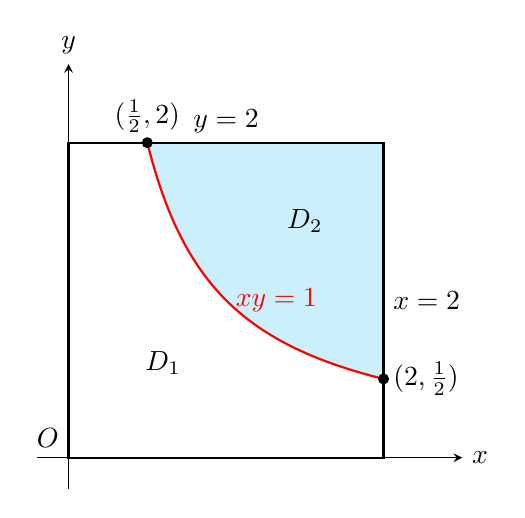
\begin{tikzpicture}[scale=2, >=stealth]
    
    % 2. 填充区域 D2 (xy > 1)
    \fill[cyan!20] (0.5,2) plot[domain=0.5:2, samples=50] (\x, {1/\x}) -- (2,0.5) -- (2,2) -- cycle;

    % 3. 画坐标轴
    \draw[->] (-0.2,0) -- (2.5,0) node[right] {$x$};
    \draw[->] (0,-0.2) -- (0,2.5) node[above] {$y$};
    \node[above left] at (0,0) {$O$};

    % 4. 画边界正方形
    \draw[thick] (0,0) rectangle (2,2);
    \draw[dashed] (2,0) -- (2,2) node[midway, right] {$x=2$};
    \draw[dashed] (0,2) -- (2,2) node[midway, above] {$y=2$};

    % 5. 画分界线 xy = 1
    \draw[thick, red, domain=0.5:2, samples=100] plot (\x, {1/\x});
    \node[red, right] at (1,1) {$xy=1$};

    % 6. 标注区域文字
    \node at (0.6, 0.6) {$D_1$};
    \node at (1.5, 1.5) {$D_2$};

    % 7. 标注关键交点
    \fill (2,0.5) circle (1pt) node[right] {$(2, \frac{1}{2})$};
    \fill (0.5,2) circle (1pt) node[above] {$(\frac{1}{2}, 2)$};

\end{tikzpicture}
\end{document}